\section{Multimodal PET/CT Tumour
Segmentation and Prediction of
Progression-Free Survival using a
Full-Scale UNet with Attention}

\subsection*{Ссылка} \url{https://arxiv.org/abs/2111.03848}
\subsection*{Введение}
Опухоли головного мозга и шеи являются пятыми по распространенности 
онкологическими заболеваниями в мире. Сегментация новообразований 
в области головы и шеи и предсказание исхода болезни важны 
для диагностики, лечения и мониторинга заболевания.Ручная сегментация
новообразований, локализованнных в голове и шее является более сложной задачей по 
сравнению с другими частями тела, потому что опухоль показывает похожие 
значения интенсивности с соседними тканями, и человеческому глазу трудно отделить 
больную ткань от здоровой по КТ-изображению. На данный момент комбинация ПЭТ/КТ 
играет ключевую роль в диагностике новообразований. В данной работе
решается задача сегментации опхолей головы и шеи с помощью 
сверточной нейронной сети, а также задача предсказания выживаемости пациентов с помощтб 
регресионной модели.
\subsection*{Основная идея}
Авторы предлагают производить сегментацию опухолей головы и шеи по ПЭТ/КТ 
изображениям, используя полномасшатбную сеть архитектуры 3D UNet3++ с механизмом,
имитирующим когнитивное внимание (attention mechanism).  Предложенная модель, 
NormResSE-UNet3+ была обучена с гибридной функцией потерь, состоящей из Log Cosh Dice и Focal loss. 
Далее, предсказанные карты сегментации дополнительно уточняются с помощью механизма постпроцессинга -
Conditional Random Fields, чтобы уменьшить число ложноположительных ответов 
и улучшить сегментацию границы опухоли. Для решения задачи предсказания 
выживаемости предлагается регресионная модель CoxPH относительной опасности, использующая 
комбинацию клинических, radiomics (признаки, полученные из медицинских изображений с помощью определенных методов) признаков, а также признаков, полученных при глубоком обучении на ПЭТ/КТ-изображениях.
\subsubsection*{Предобработка данных}
Для задачи сегментации была использована трилинейная интерполяция (trilinear interpolation) ПЭТ и КТ-изображений.
Интесивность ПЭТ (заданная в SUV) была нормализована с помощью Z-score, а интенсивность КТ (заданная по шкале Хаунсфилда), 
приведена к [-1,1]. \par
Данные для предсказания выживаемости были обработаны с учетом пропущенных значений. Каждый пропущенный признак - 
это функция от существующих признаков. Пропущенные признаки восстанавливаются итеративно
с помощью Lasso регрессии и 5-fold кросс-валидации на клинических, радиомических признаках и признаках, полученных из 3D-UNet.



\begin{minipage}{1.0\linewidth}
    \begin{center}
    
    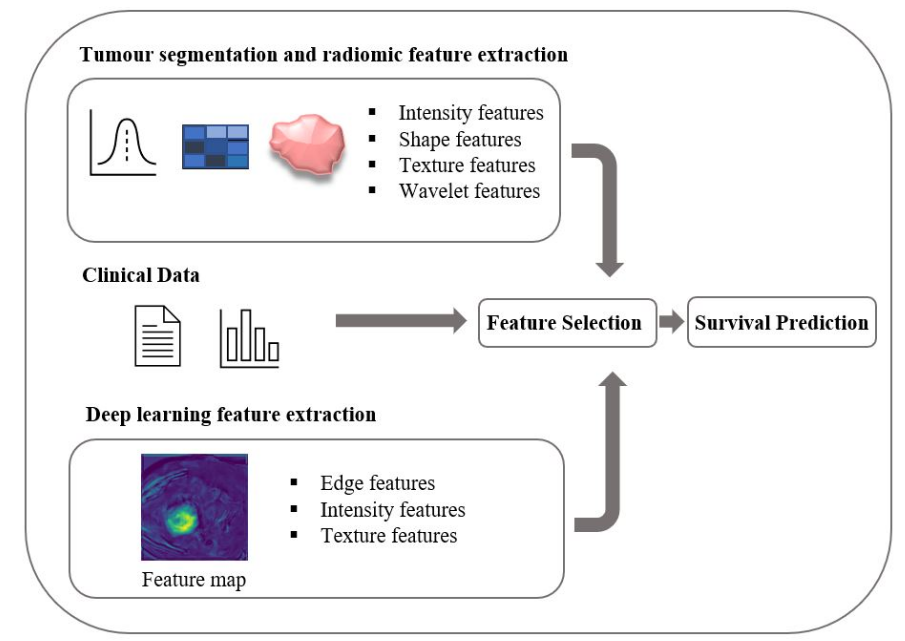
\includegraphics[scale=0.49]{annot6_features.jpg}
    \captionof{}{Пайплайн для задачи предсказания выживаемости. Состоит из трех шагов:
    сбор клинических данных, изображений и препроцессинга. Затем, выбираются извлеченные признаки и производится 
    предсказание выживаемости.}
\end{center}
\end{minipage}


\subsubsection*{Модель для сегментации}
Архитектура предложенной сети NormResSE-UNet3+: 
\begin{itemize}
    \item На вход подается тензор, размерности 2x144x144x144, состоящий из конкатенации
    ПЭТ и КТ изображений.
    \item Энкодер состоит из residual squeeze-and-excitation блоков, первый блок из которых 
    содержит 24 фильтра. Размерность выхода энкодера - 384x3x3x3
    \item Путь декодирования состоит из полномасштабных соединений и модуля, содержащего 
    правильную разметку изорбражений (ground truth).
    \item У декодера одноканальный выход размерности 1х144х144х144
\end{itemize}



    \begin{minipage}{1.0\linewidth}
        \begin{center} 
        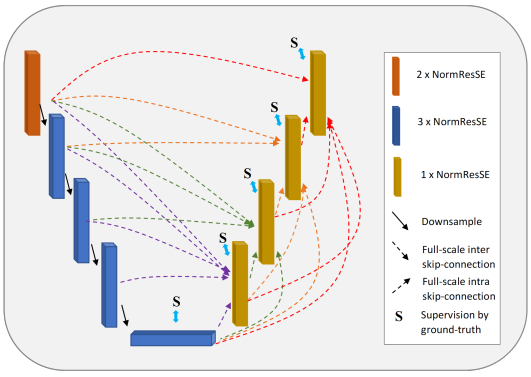
\includegraphics[scale=0.5]{ann6_arch.png}
     \end{center}

    \end{minipage}

\subsection*{Данные}
Данные были предоставленны организаторами соревнования HECTOR - MICCAI. Всего 
тренировочных примеров - 224 из 5 центров: CHGJ, CHMR, CHUS,CHUP,CHUM.

\subsection*{Результаты}
Было обучено несколько моделей нейронных сетей для задачи сегментации опухолей головы и шеи. 
Результаты сведены в единую таблицу.
\begin{minipage}{1.0\linewidth}
    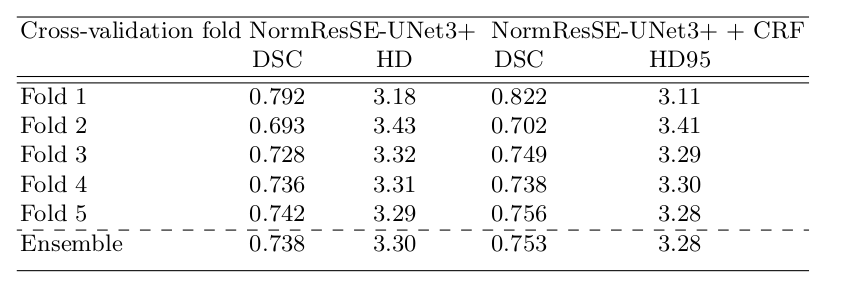
\includegraphics[scale=0.5]{ann6_res.png}
\end{minipage}
\\

Результаты предсказания выживаемости. Предложенная регрессионная модель CoxPH показала 
лучший результат: \\
\begin{minipage}{1.0\linewidth}
    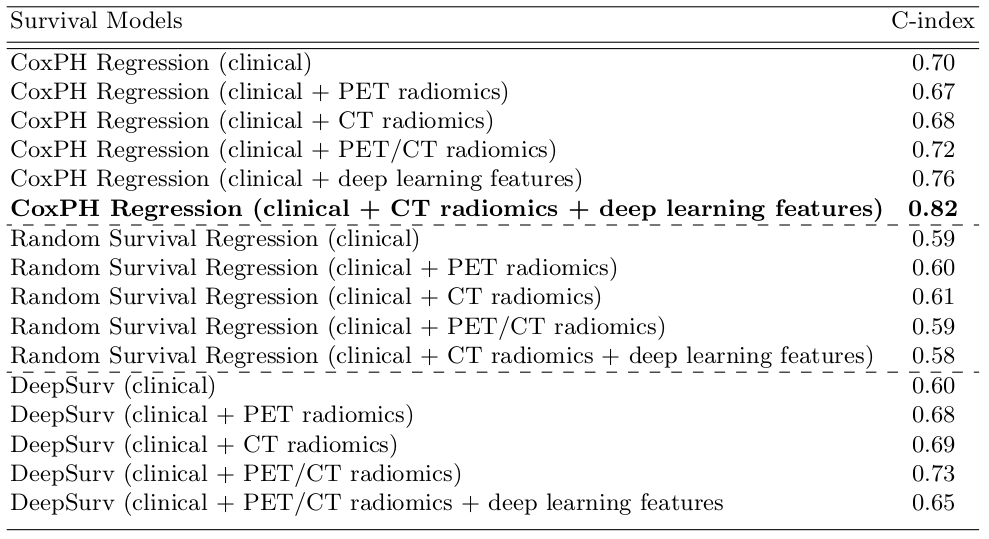
\includegraphics[scale=0.5]{ann6_reg_res.png}
\end{minipage}


\subsection*{Заключение}
Авторы предложили модель NormResSE-UNet3+ для сегментации опухолей головы и шеи по мультимодальным 
ПЭТ/КТ изображениям, в основе которой лежит архитектура UNet3+ с комбинированными слоями 
сжатия (squeeze-and-excitation), чтобы использовать возможности модели непрерывно фокусироваться 
на релевантных областях интереса, что помогло улучшить точность сегментации.
